%====================================
% Titre                  : Article sur les liens RELAX et KAOS, SEAMS version (6p.)
% File Name              : SEAMS.tex
% Copyright (C) 2011 par : M. AHMAD & J-M. BRUEL
% Last Update            : $Id$
%====================================

%------------------------------------------------------
\documentclass[10pt, conference, compsocconf]{IEEEtran}

% Definitions
\def\myrelax{\textsc{Relax}}                  % TradeMarks
\def\sysml{\textsc{SysML}}
\def\topcased{\textsc{Topcased}}
\def\kaos{\textsc{Kaos}}
\newcommand{\Mysec}[1]{section~\ref{sec:#1}}
\newcommand{\Myfig}[1]{Figure~\ref{fig:#1}}
\newcommand{\stereotype}[1]{\textless\textless\texttt{#1}\textgreater\textgreater}

% *** GRAPHICS RELATED PACKAGES ***
%
\ifCLASSINFOpdf
  \usepackage[pdftex]{graphicx}
  \DeclareGraphicsExtensions{.pdf,.jpeg,.png}
\else
  \usepackage[dvips]{graphicx}
  \DeclareGraphicsExtensions{.eps}
\fi

% correct bad hyphenation here
%\hyphenation{op-tical net-works semi-conduc-tor}

\pagestyle{plain}

\begin{document}
%
% paper title
% can use linebreaks \\ within to get better formatting as desired
\title{Using RELAX and KAOS for Adaptive Systems Requirements Modeling}


% author names and affiliations
% use a multiple column layout for up to two different
% affiliations

\author{\IEEEauthorblockN{Manzoor Ahmad and Jean-Michel Bruel}
\IEEEauthorblockA{University of Toulouse\\
	CNRS/IRIT\\
	F-31062 Toulouse Universit\'e Cedex, France\\
       Email: \{manzoor.ahmad,bruel\}@irit.fr}
\and
\IEEEauthorblockN{R\'egine Laleau and Christophe Gnao}
\IEEEauthorblockA{line 1 (of Affiliation): dept. name of organization\\
line 2: name of organization, acronyms acceptable\\
line 3: City, Country\\
line 4: Email: name@xyz.com}
}


% make the title area
\maketitle

%------------------------------------------------------
\begin{abstract}
Dynamic Adaptive Systems (DAS) modify their behavior at run-time in response to 
changing environmental conditions. For these systems, non-functional requirements play an 
important role, and one has to identify requirements that are concerned with the adaptive 
features.  Goal based approaches can help in the development of requirements for DAS, keeping in view the inherent uncertainty in these systems. \myrelax{}, which is a requirement engineering language, can introduce flexibility in 
non-functional requirements to adapt to any changing environmental conditions. 
This paper shows how to model adaptive systems requirements through an existing goal 
oriented approach that extends the \sysml{} meta-model and our proposed domain 
specific language for \myrelax{}, that enables to derive requirements in graphical 
format from textual requirements in the form of \sysml{} requirements diagrams. 
Moreover, a merge of the two approaches will serve the development of DAS.
\end{abstract}
%------------------------------------------------------

\begin{IEEEkeywords}
Domain Specific Language; RELAX; Integrated Development Environment; Dynamic Adaptive Systems; Requirements Engineering;

\end{IEEEkeywords}


% For peer review papers, you can put extra information on the cover
% page as needed:
% \ifCLASSOPTIONpeerreview
% \begin{center} \bfseries EDICS Category: 3-BBND \end{center}
% \fi
%
% For peerreview papers, this IEEEtran command inserts a page break and
% creates the second title. It will be ignored for other modes.
\IEEEpeerreviewmaketitle


%------------------------------------------------------
\section{Introduction}
%------------------------------------------------------

Most of the work in Requirements Engineering (RE) for Dynamic Adaptive Systems (DAS) assume that requirements already exists and their main focus is on requirements monitoring and reasoning about the correctness of adaptations [1]. The environmental conditions for these systems tend to change so they have to adapt to these changing conditions.  In other words, we can say that DAS tend to be cyber-physical systems where the physical environment is tightly intertwined with the computing based system. 

Goals can be used to systematically model the requirements of a DAS, they are treated as a collection of target systems with varying environmental conditions, so each target system's requirements are modeled and the adaptive logic that serves for the transition between the configurations are treated as separate concerns [2]. To develop goal models, a process can be used called LOREM ( Levels Of Requirement Engineering for Modeling) [3], to represent the individual target system and the adaptive logic. 

Our previous work [4] with requirements serve as a baseline for using \myrelax{} [5] to model non-functional requirements. \myrelax{} is a textual programming language which deals with uncertainty in DAS requirements which allows requirements to be temporarily relaxed to adapt to changing environmental conditions. This relaxation is offered in case non-critical requirements be partially neglected in order to satisfy short term critical requirements. The distributed nature of DAS and changing environmental factors make it difficult to anticipate all the explicit states in which the system will be during its life time. As such a DAS needs to be able to tolerate a range of environmental conditions and contexts, but the exact nature of these contexts remains imperfectly understood. One overarching challenge in developing DAS, therefore, is how to handle the uncertainty posed by the respective application domains. 

We can take benefits from goal oriented approaches in defining requirements for self adaptive systems. The worth of goal oriented techniques for requirements engineering in general can be found in literature [6] [7]. 

The context of our work is situated in Autonomic Computing where we are working on a case study of an AAL (Ambient Assisted Living) house [5]. The case study highlights the need to ensure patient's health in the AAL house. This house is equiped with an intelligent fridge that communicates with the AAL and is capable of reading, storing RFID information on food items. It also comes with 4 temperature and 2 humidity sensors. The fridge also detects the presence of spoiled food and discovers and receives a diet plan to be monitored based on what food items the patient is consuming. 


The rest of the paper is organized as follows: \Mysec{Our Previous Work} shows the motivations of our work, background of the concepts, our previous experience, some challenges we are facing and the limitations of our work; \Mysec{contrib} shows why use goals for defining requirements, the integration of goals in defining requirements  for DAS, their benefits and the relationship between different concepts and \Mysec{Conclusion and Future Work} concludes the paper with an insight on the future work.

%------------------------------------------------------
\section{Our Previous Work}\label{sec:Our Previous Work}
%------------------------------------------------------

\subsection{Motivations}

Our primary motivation is to enforce three aspects of the DAS requirements engineering:
\begin{itemize}
\item to ease the identification of those requirements on which the adaptation is going to apply (this is our primary work around \myrelax{} [5])
\item their traceability through the development life cycle (this is our primary work around \sysml{} [8])
\item to integrate goal oriented  concepts in defining requirements for DAS
\end{itemize}

We have focussed so far on the requirements themselves (individually), the way we can write them in a more useful and precise way (see \Myfig{relaxreq}), and the way we can automatically inject them in a system model (see \Myfig{reqdiag}).
The next step is now to work on the way we can identify the requirements that can be relaxed (called "relaxable") or not.
This is why we are currently investigating the use of goal based approaches.

%------------------------------------------------------
\begin{figure}[!t]
\centering
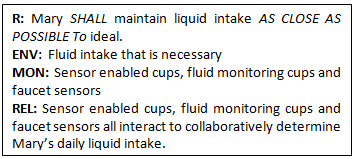
\includegraphics[width=3.4in]{fig15}
\caption{A requirement using the RELAX syntax [5]}
\label{fig:relaxreq}
\end{figure}
%------------------------------------------------------

\subsection{SysML}


\sysml{}\footnote{http://www.sysml.org/specs/} is a general purpose modeling language for systems engineering applications. It supports the specification, analysis, design, verification and validation of a broad range of systems and systems-of-systems. These systems may include hardware, software, information, processes, personnel, and facilities. It includes a graphical construct to represent text based requirements and relate them to other model elements. The requirements diagram captures requirements hierarchies and requirements derivation, and the satisfy and verify relationships allow a modeler to relate a requirement to a model element that satisfies or verifies the requirements. The requirement diagram provides a bridge between the typical requirements management tools and the system models.

\subsection{RELAX}

Typical textual requirements use modal verb SHALL that defines the functionality that a software system must always provide. \myrelax{} takes the form of structured natural language, including operators designed specifically to capture uncertainty [9], their semantics is also defined. Uncertainty can be environmental and behavioral; environmental uncertainty is due to the changing environmental conditions such as sensor failure, noisy networks, malicious threats and unexpected human input, here uncertainty refers to maintaining the same requirements in unknown contexts whereas behavioral uncertainty refers to situations where requirements themselves need to change.

The \myrelax{} vocabulary helps in relaxing requirements when environment changes so it enables the analysts to identify the point of flexibility in their requirements. For this purpose \myrelax{} process [5] is used which divides requirements into two types: variant or relaxed requirements that can be relaxed when the environment changes and invariant requirements that are fixed and cannot be changed keeping in view that it is the main functionality of the system. The relaxation also implies that a trade-off be made between critical and non-critical requirements when the environment changes, or resources are constrained, in such a case, we can compromise non-critical requirements for critical requirements. 

In \myrelax{} the conventional modal verb SHALL is retained and \myrelax{} operators are introduced to provide more flexibility in how and when that functionality may be delivered. More specifically, for requirements that are left partially unsatisfied, the introduction of an alternative, temporal or ordinal \myrelax{}-ation modifier will define the requirement as \myrelax{}-able. These operators define constraints on how a requirement can be relaxed at run-time. In addition, it is important to indicate what uncertainty factors warrant a relaxation of these requirements, thereby requiring adaptive behavior. This information is specified using the MON (monitor), ENV (environment), REL (relationship) and DEP (dependency) keywords.

\sysml{} incorporates requirements through requirements diagram so a link between \sysml{} and \myrelax{} would help in modeling the requirements efficiently. \sysml{} provides a development environment and a graphical support for expressing all the variables of \myrelax{} and also it helps in bridging the gap between the requirements and the overall system model as it is becoming an industry standard.

%------------------------------------------------------
\begin{figure}[!t]
\centering
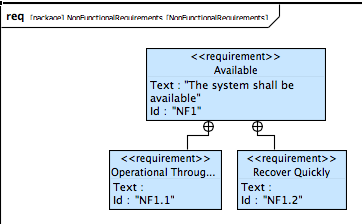
\includegraphics[width=2.5in]{fig4}
\caption{Generated Requirements Diagram}
\label{fig:reqdiag}
\end{figure}
%------------------------------------------------------

\subsection{DSL for RELAX}

Our previous work with \myrelax{} is centered on a Domain Specific Language for self adaptive systems [4]. \myrelax{} grammar is used as a meta-model for our DSL and based on this meta-model we would be able to bridge the gap between requirements and the overall system model. 

Using our DSL [4], non-functional requirements in textual format are transformed into graphical format with the help of \myrelax{} grammar in the form of requirements diagram. \Myfig{reqdiag} shows a snapshot of the generated requirements diagram.  



For the generation of DSL, XText\footnote{http://www.eclipse.org/Xtext/documentation} is used. XText is a development framework for the development of DSL and other textual programming languages and helps in the development of an  Integrated Development Environment (IDE) for the DSL. Some of the IDE features that are either derived from the grammar or easily implementable are: syntax coloring, outline view, model navigation, code completion and code templates. Among the benefits of XText, we have benefited from the code generation framework that is automatically generated from the grammar. A code generator has been written that is capable of processing models created with the DSL editor [8]. 


As a more perspective contribution a tool, COOL \myrelax{} Editor [10] is developed using \myrelax{} grammar as a meta-model. It is developed with all the \myrelax{} variables embedded in it and with the help of this tool we can do M2T (Model 2 Text) and M2M (Model 2 Model) transformation. 

\subsection{SysML/KAOS}

%\kaos{} is a method for RE which is the result of the work performed in University of Louvain [11], that enables analysts to build requirements models and to derive requirements documents from \kaos{} models. \kaos{} is goal driven: having identified a few preliminary goals for a system-to-be, the %\kaos{} framework facilitates the identification of further goals – and the requisites, objects, agents and actions of the system. A \kaos{} model aggregates four complementary and interrelated views on the information system [12]. \Myfig{KAOS} shows the four \kaos{} models.




%------------------------------------------------------
\begin{figure}[!t]
\centering
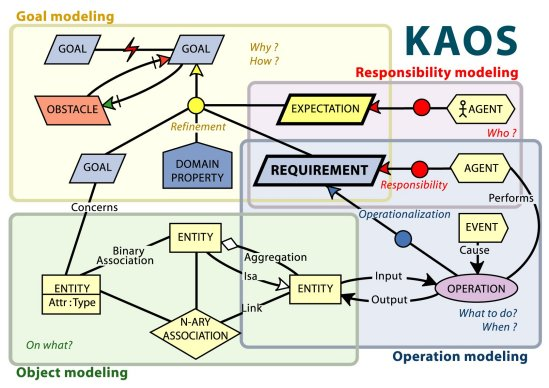
\includegraphics[width=3.4in]{fig7}
\caption{KAOS Models [12]}
\label{fig:KAOS}
\end{figure}
%------------------------------------------------------


%\sysml{} meta-model is extended with the goal concept i.e. with \kaos{} [13]. Although \sysml{} has a set of concepts regarding requirements but the basic idea behind this extension is that they are not very rich as compared to other methods of RE. In \sysml{}, the notion of requirements is %defined in an informal way and only through textual form and the relation between requirements does not have a precise semantics which results in confusion. The \sysml{} extension is possible through UML profiling [14].  


%The yellow boxes in \Myfig{meta} shows the \sysml{}/\kaos{} concepts and the grey boxes shows the \sysml{} concepts. By instantiating this meta-model, we obtain a hierarchy of non-functional requirements in the form of non-functional goals. The meta-class NON FUNCTIONAL GOAL %represents the non functional goal, it is specified as a sub-class of the meta-class GOAL which itself is a sub-class of the meta-class REQUIREMENT of \sysml{}.  


%------------------------------------------------------
\begin{figure*}[!t]
\centering
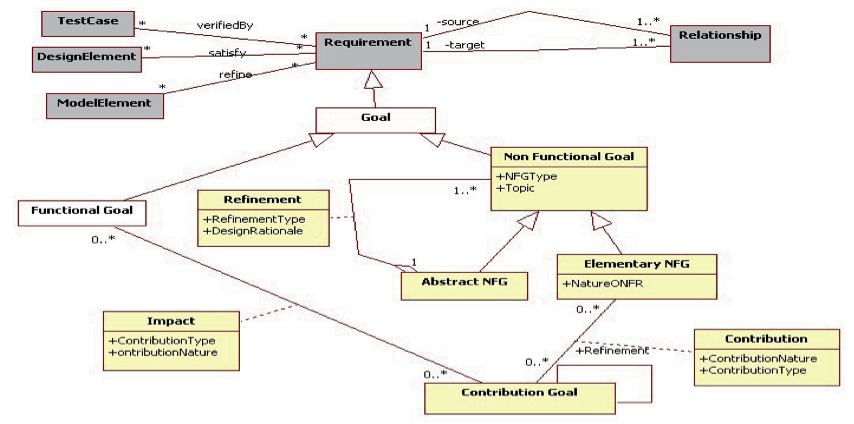
\includegraphics[width=5.5in]{fig5}
\caption{Extended SysML Meta-Model [13]}
\label{fig:meta}
\end{figure*}
%------------------------------------------------------

\subsection{Current Limitations}





%------------------------------------------------------
\section{Our Contribution in Requirements Modeling}\label{sec:contrib}
%------------------------------------------------------

% Overall process starting from textual requirements to the generation of requirements diagrams, parametric diagrams on one hand and improvements frol KAOS positive/negative, direct/indirect impacts plus the correlation at the MM level.

\subsection{The Overall Process}

\Myfig{Workplan} shows the integrated work plan.

An excerpt of the case study is given below: 
Mary is a widow. She is 65 years old, overweight and has high blood pressure and cholesterol levels. Following her doctor's instructions, she is considering to lose weight. The doctor has recommended a hypo caloric diet with low levels of salt. She lives by herself in an AAL house.


For the correspondence between requirement and goal, we know that a \stereotype{Block} satisfy \stereotype{Requirement} and an \stereotype{Agent} satisfy \stereotype{Goal}, so we can deduce a hypothesis from this correlation that a \stereotype{Requirement} corresponds to a \stereotype{Goal} and a \stereotype{Block} corresponds to an \stereotype{Agent}. This hypothesis can be verified by the work of Chung [15] and Cysneiros [16] which shows that non functional requirements can be formulated in the form of goals. 

Based on our experience with the AAL case study, we can deduce that requirement corresponds to goal. \Myfig{ReqDiag} shows the SysML requirement diagram. Here the main requirement is to keep mary healthy; this requirement is composed of two requirements i.e. \stereotype{Minimum liquid intake} which is satisfied by the block \stereotype{Sensor enabled cups} and \stereotype{Hypo caloric diet} which is satisfied by the block \stereotype{Fridge display}. \Myfig{KAOSModel} shows the \kaos{} responsibility model: here the main goal is to look after the mary diet plan which is decomposed into two sub goals. The first sub goal is the \stereotype{Minimum liquid intake} which is achieved by the agent \stereotype{Sensor enabled cups} and the other sub goal is \stereotype{Hypo caloric diet} which is achieved by the agent \stereotype{Fridge display}.  

Uncertainty factors especially ENV and MON attributes are particularly important for documenting whether the system has the means for monitoring the important aspects of the environment. By collecting these ENV and MON attributes, we can build up a model of the environment in which the system will operate, as well as a model of how the system monitor its environment. Having said this, \sysml{}/\kaos{} can complement \myrelax{} by injekting more information in the form of positive/negative and direct/indirect impacts. 

%------------------------------------------------------
\begin{figure}[!t]
\centering
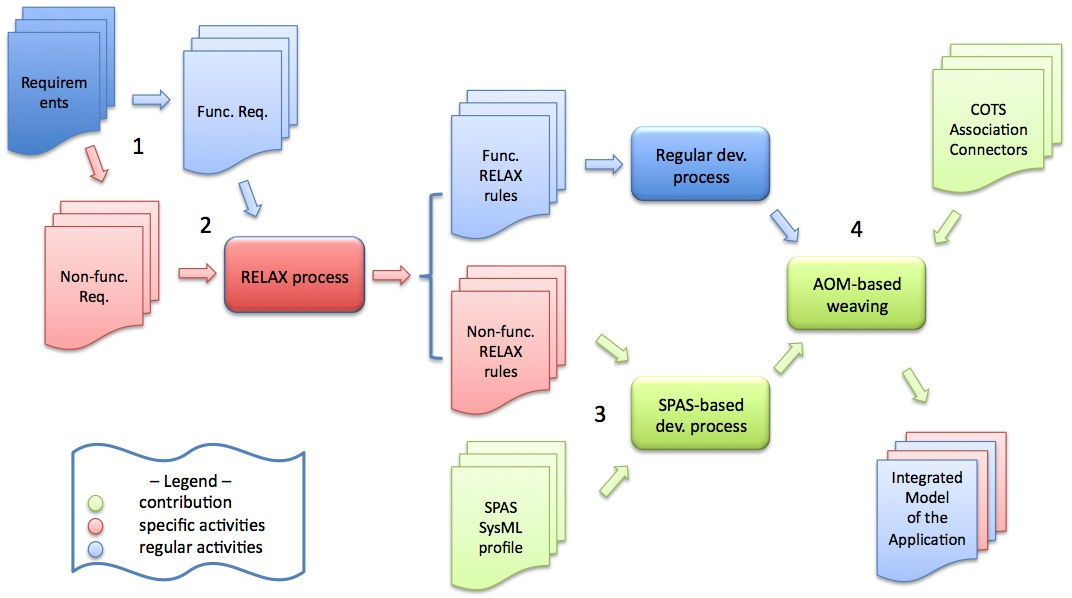
\includegraphics[width=3.5in]{fig1}
\caption{Integrated Work Plan}
\label{fig:Workplan}
\end{figure}
%------------------------------------------------------

\subsection{Why Use Goal Oriented Techniques for Requirements Engineering}

% To be added

%------------------------------------------------------
\begin{figure}[!t]
\centering
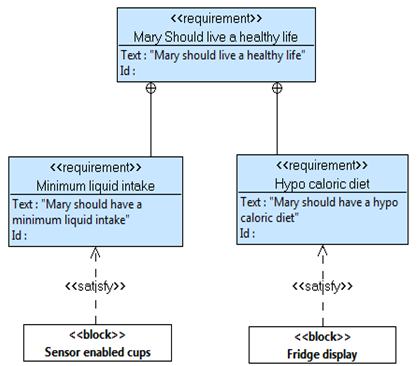
\includegraphics[width=2.5in]{fig14}
\caption{SysML Requirement Diagram}
\label{fig:ReqDiag}
\end{figure}
%------------------------------------------------------

%------------------------------------------------------
\begin{figure}[!t]
\centering
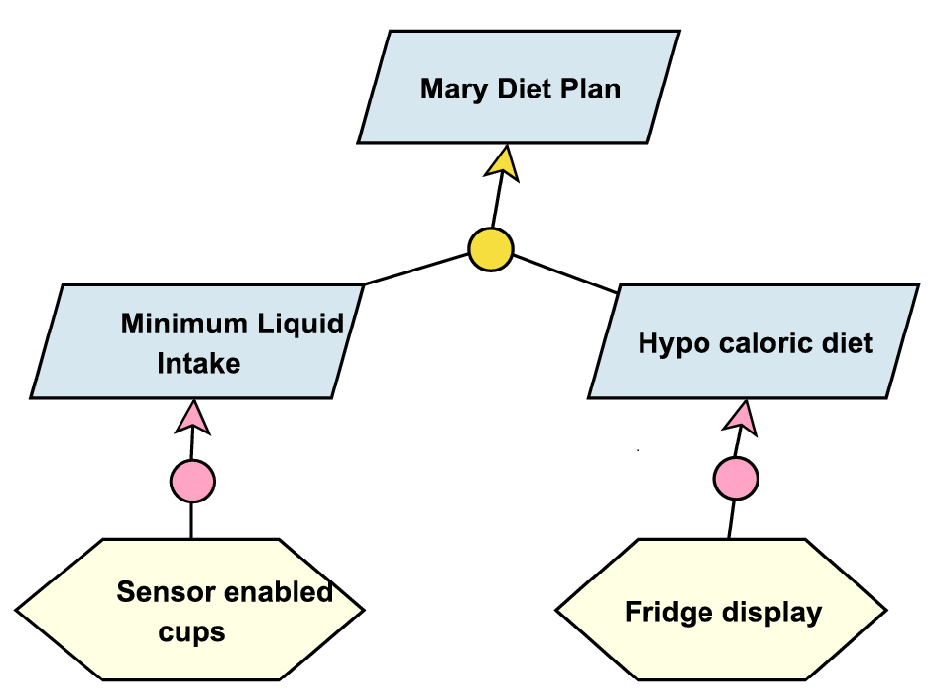
\includegraphics[width=2.5in]{fig12}
\caption{KAOS Responsibility Model}
\label{fig:KAOSModel}
\end{figure}
%------------------------------------------------------

\subsection{Relationship b/w SysML/KAOS, SysML and RELAX}

In \Myfig{Relationship} we have studied how several key concepts are taken into account in the selected models. Most of the time, the concepts are not fully covered (e.g. \stereotype{satisfy} for monitoring in \sysml{}, this stereotype is used between a block and a requirement), but we have indicated in the table the closest mechanism that supports the concepts. In \sysml{}/\kaos{}; requirements are described in the form of goals, \sysml{} describes requirements in textual form while \myrelax{} requirements are also in textual form with an enhanced version i.e. requirements divided into invariant and \myrelax{}-ed requirements with uncertainty factors added to it. \sysml{}/\kaos{} has no AND/OR refinement relationships, \sysml{} has \stereotype{verify} and \stereotype{refine} relationships while for \myrelax{} we have REL variable which identifies the relationship between ENV and MON. For Dependency/Impact \sysml{}/\kaos{} deals with it as the impact of non-functional goal on functional goal; this impact can be positive or negative and direct or indirect while for \sysml{}/ we have the concept of \stereotype{derive} which shows the dependency between requirements, \myrelax{} has positive and negative dependency. To deal with monitoring \sysml{}/\kaos{} has the \stereotype{contribution goal} concept which is used to satisfy a non-functional goal, \sysml{} has \stereotype{satisfy} which is  used when a \stereotype{block} satisfies a \stereotype{requirement} while for \myrelax{} we have the concept of MON which is used to measure the environment i.e. ENV. \sysml{}/\kaos{} has a tool called \sysml{}/\kaos{} editor, \sysml{} has a number of tools e.g. eclipse\footnote{http://www.eclipse.org/}, papyrus\footnote{http://www.papyrusuml.org}, topcased\footnote{http://www.topcased.org/} etc and for \myrelax{} we have eclipse based COOL \myrelax{} editor [10]. 

%------------------------------------------------------
\begin{figure}[!t]
\centering
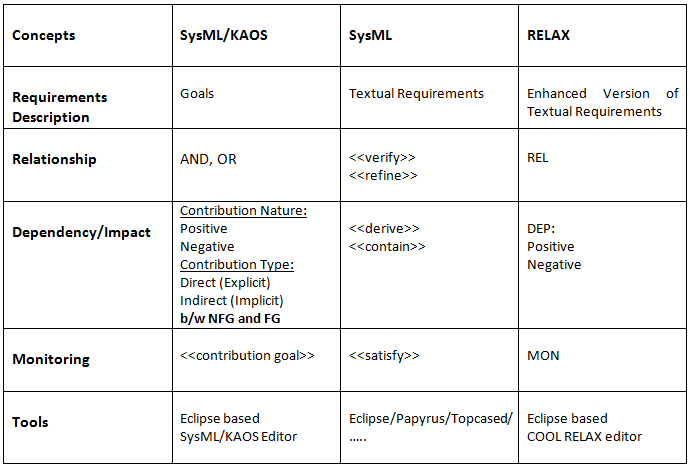
\includegraphics[width=3.4in]{fig13}
\caption{Relationship b/w Different Concepts}
\label{fig:Relationship}
\end{figure}
%------------------------------------------------------

%------------------------------------------------------
\section{Conclusion and Future Work}\label{sec:Conclusion and Future Work}
%------------------------------------------------------

Dynamic adaptive systems modify their behavior at run-time in response to changing environmental conditions. For these systems, non-functional requirements play an important role, and one has to identify requirements that are concerned with the adaptive features. For the development of requirements for DAS, goal based approaches play an important role keeping in view the inherent uncertainty in these systems. \myrelax{} which is a RE language for self-adaptive systems can introduce flexibility in non-functional requirements; to adapt to any changing environmental conditions. This paper is based on requirements modeling using two different approaches: one through the use of existing goal oriented approach, for which \sysml{} meta-model is extended with the goal concepts and the other proposed approach use \myrelax{} which takes requirements in textual format and transform it into graphical format using \myrelax{} grammar that acts as a meta-model. 

We are of the view that \sysml{}/\kaos{} can help \myrelax{} inject more information in the form of positive/negative and direct/indirect impacts. Our work on \myrelax{} is a part of an integrated work plan [17].  Our work and \sysml{}/\kaos{} approach treat requirements from the very beginning and also the uncertainty that is surrounding self-adaptive systems. This work is a baseline for more concrete work as to explore fully the merging, the challenges related to this integration. In itself, integrating many modeling languages (\kaos, \sysml{} and \myrelax{}) is probably a good idea, as each of these languages brings its own analysis and has its own benefits. Another important aspect of \myrelax{} is that the ENV, MON and REL attributes will be particularly interesting in building the SysML parametric diagrams so we can for example use mathematical equations to implement these attributes in the parametric diagram. Futrure work is centered around the development of the AAL case study. We are also interested in using formal methods to prove that whether certain properties are complementary with each other or not even before development. As an AAL house contains different technologies ranging from medical services to surveillance cameras to intelligent devices e.g refrigerators etc., so using formal methods like B will greatly help in proving different properties. 
% conference papers do not normally have an appendix


%------------------------------------------------------
\section*{Acknowledgment}
%------------------------------------------------------

The authors would like to thank their M.Sc. students for the COOL tool they have developed \cite{test10}.


\begin{thebibliography}{1}
\bibitem{test1}
B. H. C. Cheng, P. Sawyer, N. Bencomo, J. Whittle. A Goal-Based Modeling Approach to Develop Requirements of an Adaptive System with Environmental Uncertainty, MODELS '09 Proceedings of the 12th International Conference on Model Driven Engineering Languages and Systems Denver Colorado USA October 4-9, 2009, Springer-Verlag Berlin, Heidelberg 2009 ISBN: 978-3-642-04424-3.
\bibitem{test2}
J. Zhang, B. H. C. Cheng, Model-based development of dynamically adaptive software, ICSE 06: Proceedings of the 28th international conference on Software engineering, New York USA, ACM (2006) 371 - 380.
\bibitem{test3}
H. Goldsby, P.  Sawyer, N. Bencomo, D. Hughes, B. H. C. Cheng, Goal-based modeling of dynamically adaptive system requirements, 15th Annual IEEE Int. Conf. on the Engineering of Computer Based Systems (ECBS) 2008.
\bibitem{test4}
M. Ahmad, First Step towards a Domain Specific Language for Self Adaptive Systems, 10th Annual International Conference on New Technologies of Distributed Systems (NOTERE), May 31- June 2 2010 Tozeur Tunisia, P. 285 - 290 ISBN: 978-1-4244-7067-9 DOI :10.1109/NOTERE.2010.5536629.
\bibitem{test5}
J. Whittle, P. Sawyer, N. Bencomo, B. H. C. Cheng, J. M. Bruel, \myrelax{}: Incorporating Uncertainty into the Specification of Self-Adaptive systems, Proceedings of the 2009, 17th IEEE International Requirements Engineering Conference, Pages: 79-88 ISSN:1090-705X, 978-0-7695-3761-0.
\bibitem{test6}
Axel Van Lamsweerde, "Goal-Oriented Requirements Engineering: A Guided Tour", Fifth IEEE International Symposium on Requirements Engineering (RE'01) Toronto, 249-263.
\bibitem{test7}
Shahzad Anwer, Naveed Ikram, "Goal Oriented Requirement Engineering: A Critical Study of Techniques," 13th Asia Pacific Software Engineering Conference (APSEC'06), pp.121-130.
\bibitem{test8}
M. Ahmad, J. M. Bruel, Requirement Language Tooling with Xtext, UBIMOB 2011 7es Journ\'ees francophones Mobilit\'e et Ubiquit\'e Toulouse, Museum d'Histoire Naturelle 6 juin 2011 -- 8 juin 2011.
\bibitem{test9}
J. Whittle, P. Sawyer, N. Bencomo, and B. H. C. Cheng. Reassessing languages for requirements engineering of selfadaptive systems, In RE Workshop for SOCCER08, Technical Report, 2008.
\bibitem{test10}
S. Gatti, J. Geisel, S. Labondance, J. Pages, COOL \myrelax{} Editor, Internal Report M2ICE, Universit\'e de Toulouse II Le Mirail 2011.
\bibitem{test11}
A. V. Lamsweerde, Requirements Engineering: From System Goals to UML Models to Software Specifications. Wiley, 2009.
\bibitem{test12}
A \kaos{} Tutorial, V1.0  Respect-IT, 2007
\bibitem{test13}
Y. Belkaid, C. Gnaho, F. Semmak, Cr\'eation de l'\'editeur \kaos{}-\sysml{} sous Topcased, Rapport Tacos, Juillet 2010.
\bibitem{test14}
http://www.omg.org/technology/documents/profile\_catalog.htm
\bibitem{test15}
Chung et al., Non-functional Requirements in Software Engineering. Kluwer, 1999.
\bibitem{test16}
Conceptual Modeling: Foundations and Applications - Essays in Honor of John Mylopoulos (festschrift), LNCS volume 5600. Springer, 2009.  530 pp. ISBN 978-3-642-02462-7.
\bibitem{test17}
J. M. Bruel, N. Belloir, M. Ahmad, SPAS: un profil \sysml{} pour les syst\`emes auto-adaptatifs, 15\`eme Colloque National de la Recherche en IUT (CNRIUT), Lille, June 8th to June 9th, 2009.


\end{thebibliography}




% that's all folks
\end{document}
%------------------------------------------------------


